\documentclass{article}

% content/resources/templates/preamble.tex
\usepackage[margin=0.6in]{geometry}
\author{Milav Dabgar}
\usepackage{amsmath,amssymb,amsthm}
\usepackage{booktabs}
\usepackage{multirow}
\usepackage{xcolor}
\usepackage{tcolorbox}
\tcbuselibrary{breakable,skins}
\usepackage[colorlinks=true,linkcolor=blue]{hyperref}
\usepackage{titlesec}
\usepackage{enumitem}
\usepackage{tikz}
\usepackage{pgfplots}
\usepackage{circuitikz}
\usepackage[version=4]{mhchem}
\usepackage{longtable}
\usepackage{array}
\usepackage{float}
\usepackage{caption}
\usepackage{listings}

\lstset{
  basicstyle=\small\ttfamily,
  breaklines=true,
  breakatwhitespace=false,
  postbreak=\mbox{\textcolor{red}{$\hookrightarrow$}\space},
  float=false,
  numbers=left,
  numberstyle=\tiny\color{gray},
  numbersep=10pt,
  xleftmargin=2em,
  keywordstyle=\color{blue},
  commentstyle=\color{green!60!black},
  stringstyle=\color{purple},
  backgroundcolor=\color{gray!5},
  showstringspaces=false,
  tabsize=2,
  captionpos=b,
  keepspaces=true,
  columns=flexible
}

\pgfplotsset{compat=1.18}
\usetikzlibrary{shapes,arrows,positioning,calc,patterns,decorations.pathmorphing,decorations.markings,arrows.meta}

% Color scheme
\definecolor{headcolor}{RGB}{0,102,204}
\definecolor{keycolor}{RGB}{220,20,60}
\definecolor{solutioncolor}{RGB}{34,139,34}
\definecolor{mnemoniccolor}{RGB}{148,0,211}
\definecolor{codecolor}{RGB}{0,0,100}

% Spacing
\setlength{\parskip}{3pt}
\setlist[itemize]{nosep}
\setlist[enumerate]{nosep}

% Title formatting
\titleformat{\section}{\Large\bfseries\color{headcolor}}{\thesection}{1em}{}
\titleformat{\subsection}{\large\bfseries\color{headcolor}}{\thesubsection}{1em}{}

% Pandoc tightlist compatibility
\providecommand{\tightlist}{%
  \setlength{\itemsep}{0pt}\setlength{\parskip}{0pt}}

% Pandoc longtable compatibility
\newcounter{none}
\def\thenone{}


% content/resources/templates/english-boxes.tex

% Custom environments
\newtcolorbox{solutionbox}{
 breakable,
 enhanced,
 colback=solutioncolor!5!white,
 colframe=solutioncolor!75!black,
 fonttitle=\bfseries,
 title=Solution
}

\newtcolorbox{solutionboxnobreak}{
 colback=solutioncolor!5!white,
 colframe=solutioncolor!75!black,
 fonttitle=\bfseries,
 title=Solution
}

\newtcolorbox{keyformula}{
 breakable,
 enhanced,
 colback=keycolor!5!white,
 colframe=keycolor!75!black,
 fonttitle=\bfseries,
 title=Key Formula
}

\newtcolorbox{mnemonicboxenv}{
 breakable,
 enhanced,
 colback=mnemoniccolor!5!white,
 colframe=mnemoniccolor!75!black,
 fonttitle=\bfseries,
 title=Mnemonic
}

\newcommand{\mnemonicbox}[1]{%
  \begin{mnemonicboxenv}
    #1
  \end{mnemonicboxenv}
}


% Custom commands for GTU solutions
% This file defines semantic commands for consistent formatting

% Question command with automatic formatting
\newcommand{\question}[2]{%
  \section*{Question #1}%
  \textbf{#2}%
}

% OR question variant
\newcommand{\questionor}[2]{%
  \section*{Question #1 OR}%
  \textbf{#2}%
}

% Proper table environment with caption
\newenvironment{answertable}[1]{%
  \begin{table}[htbp]
  \centering
  \caption{#1}
}{%
  \end{table}
}

% Proper figure environment for diagrams
\newenvironment{answerdiagram}[1]{%
  \begin{figure}[htbp]
  \centering
  \caption{#1}
}{%
  \end{figure}
}

% Semantic markup for key terms
\newcommand{\keyword}[1]{\textbf{#1}}
\newcommand{\code}[1]{\texttt{#1}}
\newcommand{\classname}[1]{\texttt{#1}}
\newcommand{\methodname}[1]{\texttt{#1}}

% Proper quotation marks
\newcommand{\mnemonic}[1]{``#1''}


\title{Antenna and Wave Propagation (4341106) - Winter 2023 Solution}
\date{January 24, 2024}

\begin{document}
\maketitle

\questionmarks{1(a)}{3}{Define: (1) Directivity, (2) Gain, and (3) HPBW}

\begin{solutionbox}
\begin{tabulary}{\linewidth}{|L|L|}
\hline
\textbf{Parameter} & \textbf{Definition} \\ \hline
\keyword{Directivity} & Ratio of maximum radiation intensity to average radiation intensity of an antenna. \\ \hline
\keyword{Gain} & Ratio of power radiated in a particular direction to the power that would be radiated by an isotropic antenna. \\ \hline
\keyword{HPBW (Half Power Beam Width)} & Angular width where radiation intensity is half (3dB less) of the maximum value. \\ \hline
\end{tabulary}
\end{solutionbox}

\begin{mnemonicbox}
\mnemonic{"DGH: Direction Gives Half-power"}
\end{mnemonicbox}

\questionmarks{1(b)}{4}{List the properties of electromagnetic waves}

\begin{solutionbox}
\begin{tabulary}{\linewidth}{|L|L|}
\hline
\textbf{Property} & \textbf{Description} \\ \hline
\keyword{Transverse Waves} & Electric and magnetic fields are perpendicular to the direction of propagation. \\ \hline
\keyword{Velocity} & Speed of light ($3 \times 10^8$ m/s) in vacuum. \\ \hline
\keyword{No Medium Required} & Can travel through vacuum, unlike mechanical waves. \\ \hline
\keyword{Polarization} & Defined by the direction of the electric field vector. \\ \hline
\keyword{Energy Transport} & Carries energy through space. \\ \hline
\keyword{Reflection/Refraction} & Can be reflected and refracted at boundaries. \\ \hline
\keyword{Interference/Diffraction} & Exhibits wave-like properties. \\ \hline
\end{tabulary}
\end{solutionbox}

\begin{mnemonicbox}
\mnemonic{"TVNPER: Transverse Velocity No-medium Polarized Energy Reflection"}
\end{mnemonicbox}

\questionmarks{1(c)}{7}{Explain physical concept of generation of Electromagnetic wave}

\begin{solutionbox}
\textbf{Concept}: Electromagnetic waves are generated by accelerating electric charges.

\begin{answerdiagram}{Generation of EM Waves}
\begin{tikzpicture}[node distance=1.5cm, auto]
    \node [gtu block] (charge) {Accelerating Charge};
    \node [gtu block, right=of charge] (efield) {Time-varying E-Field};
    \node [gtu block, right=of efield] (hfield) {Time-varying H-Field};
    \node [gtu block, below=of efield] (wave) {Self-sustaining EM Wave};

    \draw [gtu arrow] (charge) -- node {Produces} (efield);
    \draw [gtu arrow] (efield) -- node {Generates} (hfield);
    \draw [gtu arrow] (hfield) -- (efield);
    \draw [gtu arrow] (efield) -- (wave);
    \draw [gtu arrow] (hfield) -- (wave);
    
    % Wave visualization
    \draw [thick, blue, ->] (0,-3) -- (2,-3) node[right] {E};
    \draw [thick, red, ->] (0,-3) -- (0,-1) node[above] {H};
    \draw [thick, black, ->] (0,-3) -- (1.5,-2) node[right] {Propagation};
\end{tikzpicture}
\end{answerdiagram}

\begin{itemize}
    \item \textbf{Charge Acceleration}: When electric charges accelerate (e.g., in an AC circuit), they generate changing electric fields.
    \item \textbf{Field Coupling}: Maxwell's equations state that a changing electric field produces a magnetic field, and a changing magnetic field produces an electric field.
    \item \textbf{Self-Propagation}: This mutual generation allows the fields to detach from the source and propagate through space as a wave.
    \item \textbf{Field Orientation}: $E$ and $H$ fields are perpendicular to each other and to the direction of propagation.
\end{itemize}
\end{solutionbox}

\begin{mnemonicbox}
\mnemonic{"CASES: Charge Acceleration Self-propagates Electro-magnetic Signals"}
\end{mnemonicbox}

\orquestionmarks{1(c)}{7}{Explain how electromagnetic field radiated from a center fed dipole}

\begin{solutionbox}
\textbf{Radiation Mechanism of Dipole}:

\begin{answerdiagram}{Radiation from Center-Fed Dipole}
\begin{tikzpicture}[node distance=1.5cm, auto]
    \node [gtu block] (input) {AC Input};
    \node [gtu block, right=of input] (charges) {Oscillating Charges};
    \node [gtu block, right=of charges] (fields) {Time-varying E \& H Fields};
    \node [gtu block, right=of fields] (rad) {EM Radiation};

    \draw [gtu arrow] (input) -- (charges);
    \draw [gtu arrow] (charges) -- (fields);
    \draw [gtu arrow] (fields) -- (rad);

    % Dipole sketch
    \draw [thick] (0,-2) -- (0,-1) node[midway, left] {Top Arm};
    \draw [thick] (0,-3) -- (0,-4) node[midway, left] {Bottom Arm};
    \node at (0,-2.5) {$\sim$};
    \draw [blue, thick, ->] (0.5,-2.5) arc (-90:90:0.5);
    \draw [blue, thick, ->] (0.5,-2.5) arc (90:270:0.5);
    \node [right, blue] at (1,-2.5) {Detaching Loops};
\end{tikzpicture}
\end{answerdiagram}

\begin{itemize}
    \item \textbf{Center Feeding}: An AC voltage source is applied at the center, causing current to flow back and forth.
    \item \textbf{Charge Distribution}: As current oscillates, charges accumulate at the ends of the dipole, reversing polarity every half cycle.
    \item \textbf{Field Generation}: The oscillating charges create a time-varying electric field. The current flow creates a magnetic field around the wire.
    \item \textbf{Radiation}: As the polarity reverses, the field lines pinch off and detach from the antenna, traveling outwards as electromagnetic waves.
    \item \textbf{Pattern}: Maximum radiation is perpendicular to the wire axis (broadside).
\end{itemize}
\end{solutionbox}

\begin{mnemonicbox}
\mnemonic{"CORONA: Current Oscillates, Radiation Occurs, Near-far Areas"}
\end{mnemonicbox}

\questionmarks{2(a)}{3}{Differentiate the resonant and non-resonant antennas}

\begin{solutionbox}
\begin{tabulary}{\linewidth}{|L|L|L|}
\hline
\textbf{Feature} & \textbf{Resonant Antennas} & \textbf{Non-Resonant Antennas} \\ \hline
\keyword{Length} & Integer multiple of $\lambda/2$ & Not related to wavelength (typically long) \\ \hline
\keyword{Standing Waves} & Present & Not present (Traveling waves) \\ \hline
\keyword{Impedance} & Resistive (Real) & Complex (Real + Imaginary) \\ \hline
\keyword{Bandwidth} & Narrow & Wide \\ \hline
\keyword{Example} & Half-wave dipole & Rhombic antenna \\ \hline
\end{tabulary}
\end{solutionbox}

\begin{mnemonicbox}
\mnemonic{"RESI: Resonant Exhibits Standing-waves Impedance-real"}
\end{mnemonicbox}

\questionmarks{2(b)}{4}{Explain Yagi antenna and discuss its radiation characteristics}

\begin{solutionbox}
\textbf{Yagi-Uda Antenna}: A high-gain directional antenna consisting of a driven element and parasitic elements.

\begin{answerdiagram}{Yagi-Uda Antenna Structure}
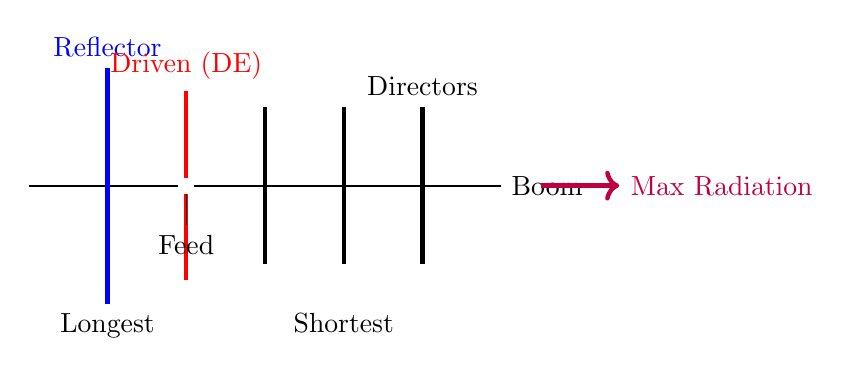
\begin{tikzpicture}
    % Boom
    \draw [thick] (0,0) -- (6,0) node[right] {Boom};
    
    % Reflector
    \draw [ultra thick, blue] (1, -1.5) -- (1, 1.5) node[above] {Reflector};
    \node [below] at (1, -1.5) {Longest};
    
    % Driven Element
    \draw [ultra thick, red] (2, -1.2) -- (2, 1.2) node[above] {Driven (DE)};
    \fill [white] (1.9, -0.1) rectangle (2.1, 0.1); % Feed gap
    \draw (2, -0.1) -- (2, -0.5) node[below] {Feed};
    
    % Directors
    \draw [ultra thick, black] (3, -1.0) -- (3, 1.0);
    \draw [ultra thick, black] (4, -1.0) -- (4, 1.0);
    \draw [ultra thick, black] (5, -1.0) -- (5, 1.0) node[above] {Directors};
    \node [below] at (4, -1.5) {Shortest};
    
    % Radiation Direction
    \draw [->, ultra thick, purple] (6.5, 0) -- (7.5, 0) node[right] {Max Radiation};
\end{tikzpicture}
\end{answerdiagram}

\begin{itemize}
    \item \textbf{Structure}: 1 Reflector (longest), 1 Driven Element ($\lambda/2$), Multiple Directors (shortest).
    \item \textbf{Directivity}: High (8-12 dB) towards the directors.
    \item \textbf{Gain}: increases with the number of directors (up to 15 dB).
    \item \textbf{Bandwidth}: Narrow (2-5\% of center frequency).
    \item \textbf{Application}: TV reception, point-to-point links.
\end{itemize}
\end{solutionbox}

\begin{mnemonicbox}
\mnemonic{"DRAGONS: Directional Reflector And Gain-improving Directors Offer Narrow Signals"}
\end{mnemonicbox}

\questionmarks{2(c)}{7}{Describe radiation characteristics of resonant wire antennas and draw the current distribution of $\lambda/2$, $3\lambda/2$ and $5\lambda/2$ antenna}

\begin{solutionbox}
Resonant wire antennas have standing wave current distributions with nodes (zero current) at the ends.

\begin{answerdiagram}{Current Distribution}
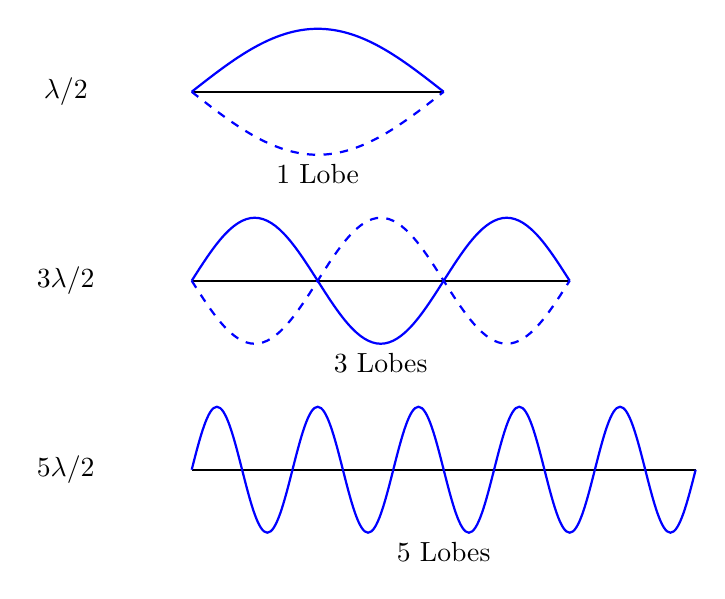
\begin{tikzpicture}[scale=0.8]
    % Lambda/2
    \node at (-2, 2) {$\lambda/2$};
    \draw [thick] (0, 2) -- (4, 2);
    \draw [thick, blue] (0, 2) sin (2, 3) cos (4, 2);
    \draw [thick, blue, dashed] (0, 2) sin (2, 1) cos (4, 2);
    \node [below] at (2, 1) {1 Lobe};

    % 3 Lambda/2
    \node at (-2, -1) {$3\lambda/2$};
    \draw [thick] (0, -1) -- (6, -1);
    \draw [thick, blue] (0, -1) sin (1, 0) cos (2, -1) sin (3, -2) cos (4, -1) sin (5, 0) cos (6, -1);
    \draw [thick, blue, dashed] (0, -1) sin (1, -2) cos (2, -1) sin (3, 0) cos (4, -1) sin (5, -2) cos (6, -1);
    \node [below] at (3, -2) {3 Lobes};

    % 5 Lambda/2
    \node at (-2, -4) {$5\lambda/2$};
    \draw [thick] (0, -4) -- (8, -4);
    \foreach \x in {0, 1.6, 3.2, 4.8, 6.4} {
        \draw [thick, blue] (\x, -4) sin (\x+0.4, -3) cos (\x+0.8, -4) sin (\x+1.2, -5) cos (\x+1.6, -4);
    }
    \node [below] at (4, -5) {5 Lobes};
\end{tikzpicture}
\end{answerdiagram}

\begin{itemize}
    \item \textbf{Half-Wave ($\lambda/2$)}: Current max at center. Radiation pattern is a simple figure-8 broadside to the wire.
    \item \textbf{$3\lambda/2$}: Three current loops. Radiation pattern splits into 3 lobes per side (6 total). Major lobes tilt towards the wire axis.
    \item \textbf{$5\lambda/2$}: Five current loops. Pattern has 5 lobes per side. As length increases, major lobes align closer to the wire axis.
    \item \textbf{General}: Number of current loops = $2L/\lambda$.
\end{itemize}
\end{solutionbox}

\begin{mnemonicbox}
\mnemonic{"NODE: Number Of Distributions Equals wavelength-multiple"}
\end{mnemonicbox}

\orquestionmarks{2(a)}{3}{Differentiate the broad side and end fire array antennas}

\begin{solutionbox}
\begin{tabulary}{\linewidth}{|L|L|L|}
\hline
\textbf{Feature} & \textbf{Broadside Array} & \textbf{End Fire Array} \\ \hline
\keyword{Max Radiation} & Perpendicular to array axis ($90^\circ$) & Along the array axis ($0^\circ, 180^\circ$) \\ \hline
\keyword{Element Spacing} & Typically $\lambda/2$ & Typically $\lambda/4$ to $\lambda/2$ \\ \hline
\keyword{Phase Difference} & $0^\circ$ (In-phase) & $180^\circ$ (Out of phase) \\ \hline
\keyword{Directivity} & High & High \\ \hline
\keyword{Pattern} & Bidirectional & Unidirectional \\ \hline
\end{tabulary}
\end{solutionbox}

\begin{mnemonicbox}
\mnemonic{"PEPS: Perpendicular Elements Produce Sideways radiation"}
\end{mnemonicbox}

\orquestionmarks{2(b)}{4}{Explain loop antenna and discuss its radiation characteristics}

\begin{solutionbox}
\textbf{Loop Antenna}: A closed circuit antenna, often circular or square.

\begin{answerdiagram}{Loop Antenna}
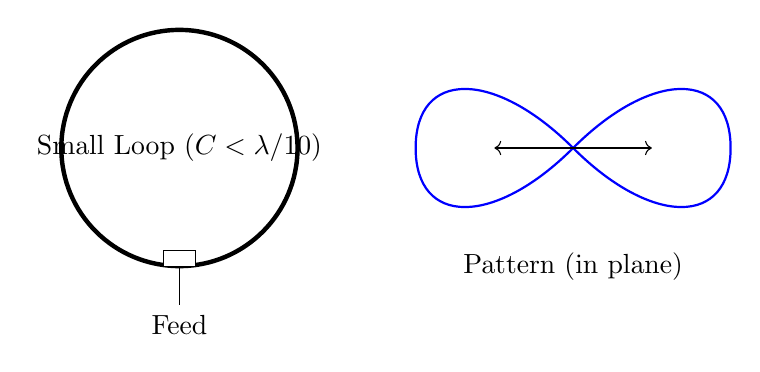
\begin{tikzpicture}
    % Small Loop
    \draw [ultra thick] (0,0) circle (1.5);
    \draw [fill=white] (-0.2, -1.5) rectangle (0.2, -1.3);
    \draw (0, -1.5) -- (0, -2) node[below] {Feed};
    \node at (0, 0) {Small Loop ($C < \lambda/10$)};
    
    % Radiation Pattern (Figure 8)
    \draw [thick, blue] (5, 0) .. controls (6, 1) and (7, 1) .. (7, 0) .. controls (7, -1) and (6, -1) .. (5, 0);
    \draw [thick, blue] (5, 0) .. controls (4, 1) and (3, 1) .. (3, 0) .. controls (3, -1) and (4, -1) .. (5, 0);
    \node at (5, -1.5) {Pattern (in plane)};
    \draw [->] (5, 0) -- (6, 0);
    \draw [->] (5, 0) -- (4, 0);
\end{tikzpicture}
\end{answerdiagram}

\begin{itemize}
    \item \textbf{Small Loop ($C < \lambda/10$)}: Acts like a magnetic dipole. Radiation pattern is a figure-8 (doughnut) similar to a short electric dipole. Pattern null is along the axis of the loop.
    \item \textbf{Large Loop ($C \approx \lambda$)}: Resonant loop. Radiation is maximum perpendicular to the loop plane (broadside).
    \item \textbf{Polarization}: Linear (Horizontal if loop is horizontal).
    \item \textbf{Applications}: Direction finding, RFID.
\end{itemize}
\end{solutionbox}

\begin{mnemonicbox}
\mnemonic{"SPIRAL: Small Patterns In Receiving And Locating signals"}
\end{mnemonicbox}

\orquestionmarks{2(c)}{7}{Describe radiation characteristics of non resonant wire antennas and draw the radiation pattern of $\lambda/2$, $3\lambda/2$ and $5\lambda/2$ antenna}

\begin{solutionbox}
Non-resonant (Traveling Wave) antennas have matched termination, so no standing waves. However, the question asks for characteristics often associated with resonant lengths in common exams, or long-wire patterns. Assuming the question implies long wire *patterns* (which are directional) or comparison with resonant. Given the specific lengths, standard resonant patterns are usually drawn.

\begin{answerdiagram}{Radiation Patterns}
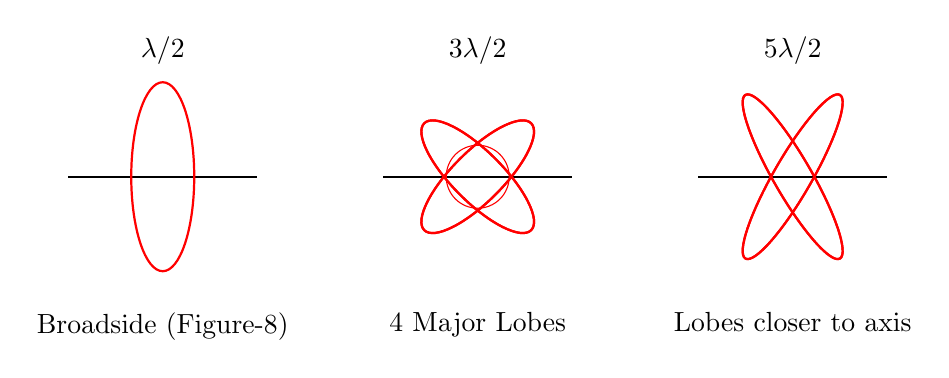
\begin{tikzpicture}[scale=0.8]
    % Lambda/2
    \begin{scope}[shift={(0,0)}]
        \node at (0, 2) {$\lambda/2$};
        \draw [thick] (-1.5, 0) -- (1.5, 0);
        \draw [thick, red] (0,0) ellipse (0.5 and 1.5);
        \node [below] at (0, -2) {Broadside (Figure-8)};
    \end{scope}

    % 3 Lambda/2
    \begin{scope}[shift={(5,0)}]
        \node at (0, 2) {$3\lambda/2$};
        \draw [thick] (-1.5, 0) -- (1.5, 0);
        \foreach \ang in {45, 135, 225, 315} {
            \draw [thick, red, rotate=\ang] (0,0) ellipse (0.4 and 1.2);
        }
        \draw [red] (0,0) circle (0.5); % Minor lobes
        \node [below] at (0, -2) {4 Major Lobes};
    \end{scope}

    % 5 Lambda/2
    \begin{scope}[shift={(10,0)}]
        \node at (0, 2) {$5\lambda/2$};
        \draw [thick] (-1.5, 0) -- (1.5, 0);
        % Simplified representation of many lobes
        \foreach \ang in {30, 150, 210, 330} {
             \draw [thick, red, rotate=\ang] (0,0) ellipse (0.3 and 1.5);
        }
        \node [below] at (0, -2) {Lobes closer to axis};
    \end{scope}
\end{tikzpicture}
\end{answerdiagram}

\begin{itemize}
    \item \textbf{$\lambda/2$}: Single major lobe perpendicular to wire (bidirectional).
    \item \textbf{$3\lambda/2$}: Major lobes shift towards the wire axis (approx $42^\circ$). Minor lobes appear broadside.
    \item \textbf{$5\lambda/2$}: Major lobes shift even closer to wire axis. More minor lobes.
    \item \textbf{Trend}: As length increases, the main beam sharpens and aligns closer to the wire axis.
\end{itemize}
\end{solutionbox}

\begin{mnemonicbox}
\mnemonic{"TWIST: Traveling Waves Increase Side-lobe Transmission"}
\end{mnemonicbox}


\questionmarks{3(a)}{3}{Write short note on micro strip (patch) antenna}

\begin{solutionbox}
\textbf{Microstrip (Patch) Antenna}: Low-profile antenna for modern applications.

\begin{answerdiagram}{Microstrip Patch Structure}
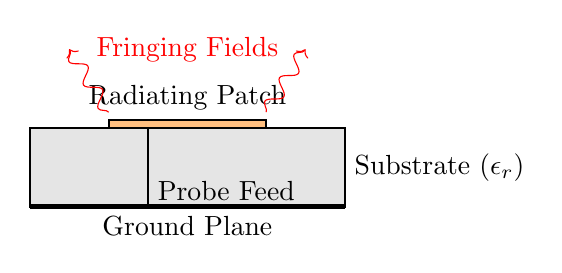
\begin{tikzpicture}
    % Substrate
    \fill [gray!20] (0,0) rectangle (4, 1);
    \draw [thick] (0,0) rectangle (4, 1);
    \node [right] at (4, 0.5) {Substrate ($\epsilon_r$)};

    % Ground Plane
    \draw [ultra thick] (0,0) -- (4, 0);
    \node [below] at (2,0) {Ground Plane};

    % Patch
    \fill [orange!50] (1, 1) rectangle (3, 1.1);
    \draw [thick] (1, 1) rectangle (3, 1.1);
    \node [above] at (2, 1.1) {Radiating Patch};
    
    % Feed
    \draw [thick] (1.5, 0) -- (1.5, 1);
    \node [right] at (1.5, 0.2) {Probe Feed};
    
    % Radiation
    \draw [->, red, decorate, decoration={snake}] (1, 1.2) -- (0.5, 2);
    \draw [->, red, decorate, decoration={snake}] (3, 1.2) -- (3.5, 2);
    \node [red] at (2, 2) {Fringing Fields};
\end{tikzpicture}
\end{answerdiagram}

\begin{itemize}
    \item \textbf{Structure}: Consists of a metallic patch on a grounded dielectric substrate.
    \item \textbf{Advantages}: Light weight, low profile, low cost, conformable to planar/non-planar surfaces.
    \item \textbf{Disadvantages}: Narrow bandwidth, low efficiency, low power handling.
    \item \textbf{Applications}: Mobile phones, GPS, missiles, satellite communications.
\end{itemize}
\end{solutionbox}

\begin{mnemonicbox}
\mnemonic{"PSALM: Patch Substrate Above Layer of Metal"}
\end{mnemonicbox}

\questionmarks{3(b)}{4}{Explain helical antenna and discuss its radiation characteristics}

\begin{solutionbox}
\textbf{Helical Antenna}: Wire wound in the form of a helix/screw, providing circular polarization.

\begin{answerdiagram}{Helical Antenna}
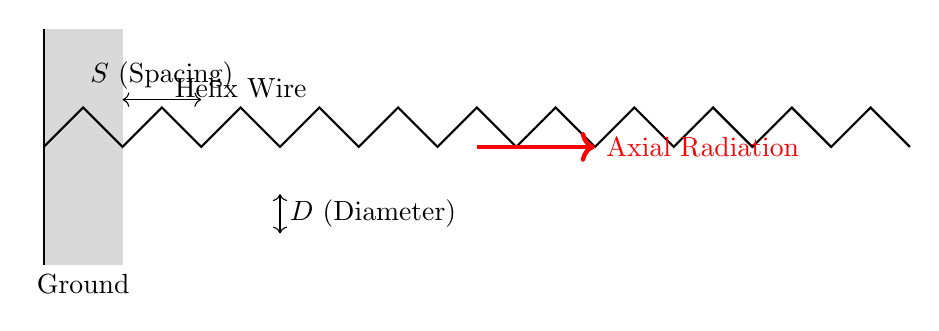
\begin{tikzpicture}
    % Ground Plane
    \fill [gray!30] (0,-1.5) rectangle (1, 1.5);
    \draw [thick] (0,-1.5) -- (0, 1.5);
    \node [below] at (0.5, -1.5) {Ground};
    
    % Helix
    \draw [thick] (0, 0) 
    foreach \x in {0, 0.5, ..., 5} {
        -- ++(0.5, 0.5) -- ++(0.5, -0.5)
    };
    \node [above] at (2.5, 0.5) {Helix Wire};
    \draw [<->] (1, 0.6) -- (2, 0.6) node[midway, above] {$S$ (Spacing)};
    \draw [<->] (3, -0.6) -- (3, -1.1) node[midway, right] {$D$ (Diameter)};

    % Radiation
    \draw [->, red, ultra thick] (5.5, 0) -- (7, 0) node[right] {Axial Radiation};
\end{tikzpicture}
\end{answerdiagram}

\begin{itemize}
    \item \textbf{Normal Mode (Broadside)}: If dimensions $<< \lambda$, radiation is perpendicular to axis. Low efficiency.
    \item \textbf{Axial Mode (End-fire)}: If Circumference $C \approx \lambda$, radiation is along the axis. High gain and Circular Polarization.
    \item \textbf{Characteristics}: Wide bandwidth (impedance remains resistive). 
    \item \textbf{Use}: Satellite tracking (due to CP).
\end{itemize}
\end{solutionbox}

\begin{mnemonicbox}
\mnemonic{"MOCHA: Mode Of Circular Helix Antennas"}
\end{mnemonicbox}

\questionmarks{3(c)}{7}{Explain horn antenna and discuss its radiation characteristics}

\begin{solutionbox}
\textbf{Horn Antenna}: Flared waveguide that matches impedance of waveguide to free space.

\begin{answerdiagram}{Horn Antenna Types}
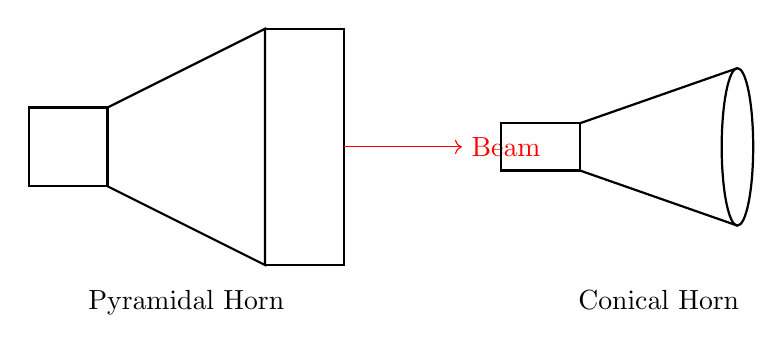
\begin{tikzpicture}
    % Pyramidal
    \draw [thick] (0,0) rectangle (1,1); % Waveguide
    \draw [thick] (1,1) -- (3,2) -- (3,-1) -- (1,0); 
    \draw [thick] (3,2) -- (4,2) -- (4,-1) -- (3,-1); % Aperture
    \draw [dashed] (0,0) -- (1,0);
    \node [below] at (2, -1.2) {Pyramidal Horn};
    \draw [->, red] (4, 0.5) -- (5.5, 0.5) node[right] {Beam};

    % Conical
    \begin{scope}[shift={(6,0)}]
        \draw [thick] (0, 0.2) rectangle (1, 0.8);
        \draw [thick] (1, 0.8) -- (3, 1.5);
        \draw [thick] (1, 0.2) -- (3, -0.5);
        \draw [thick] (3, 0.5) ellipse (0.2 and 1); 
        \node [below] at (2, -1.2) {Conical Horn};
    \end{scope}
\end{tikzpicture}
\end{answerdiagram}

\begin{itemize}
    \item \textbf{Impedance Matching}: Smooth flare minimizes reflection coefficient, reducing VSWR.
    \item \textbf{Bandwidth}: Very wide bandwidth compared to other high-gain antennas.
    \item \textbf{Directivity}: Moderate to high (10-20 dB).
    \item \textbf{Side Lobes}: Very low side lobes due to tapered aperture distribution.
    \item \textbf{Types}: Sectoral (E or H plane), Pyramidal (both planes), Conical (circular).
    \item \textbf{Application}: Feed for parabolic dishes, standard gain reference, radar.
\end{itemize}
\end{solutionbox}

\begin{mnemonicbox}
\mnemonic{"POWERS: Pyramidal Or Widening End Radiates Strongly"}
\end{mnemonicbox}

\orquestionmarks{3(a)}{3}{Write short note on slot antenna}

\begin{solutionbox}
\textbf{Slot Antenna}: A slot cut in a conductive surface.

\begin{answerdiagram}{Slot Antenna}
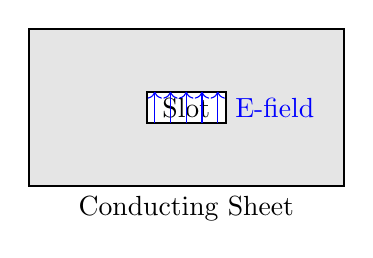
\begin{tikzpicture}
    \fill [gray!20] (0,0) rectangle (4, 2);
    \draw [thick] (0,0) rectangle (4, 2);
    \fill [white] (1.5, 0.8) rectangle (2.5, 1.2);
    \draw [thick] (1.5, 0.8) rectangle (2.5, 1.2);
    \node at (2, 1) {Slot};
    \node [below] at (2, 0) {Conducting Sheet};
    
    % E-Fields
    \foreach \x in {1.6, 1.8, 2.0, 2.2, 2.4} {
        \draw [blue, ->] (\x, 0.8) -- (\x, 1.2);
    }
    \node [blue, right] at (2.5, 1) {E-field};
\end{tikzpicture}
\end{answerdiagram}

\begin{itemize}
    \item \textbf{Babinet's Principle}: A slot antenna is the "dual" of a dipole. A horizontal slot radiates vertically polarized waves (opposite to vertical dipole).
    \item \textbf{Impedance}: Related to dipole impedance $Z_s Z_d = \frac{\eta^2}{4}$. High impedance (~500 $\Omega$).
    \item \textbf{Application}: Flush mounted on high-speed aircraft/missiles to avoid aerodynamic drag.
\end{itemize}
\end{solutionbox}

\begin{mnemonicbox}
\mnemonic{"CROPS: Complementary Radiation Opening Perpendicular to Surface"}
\end{mnemonicbox}

\orquestionmarks{3(b)}{4}{Explain parabolic reflector antenna and discuss its radiation characteristics}

\begin{solutionbox}
\textbf{Parabolic Reflector}: Converts spherical waves from a point source (focus) into plane waves (collimated beam).

\begin{answerdiagram}{Parabolic Reflector}
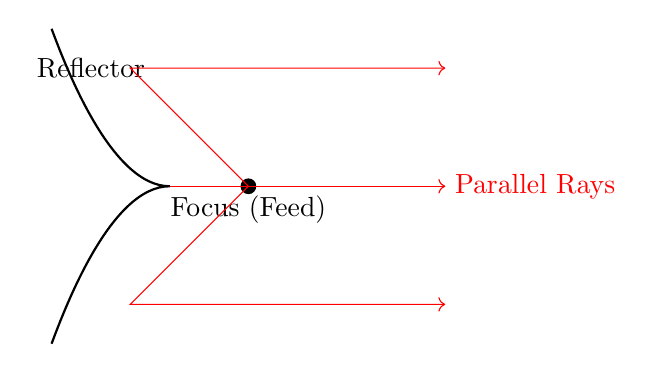
\begin{tikzpicture}
    % Parabola
    \draw [thick] (0, -2) parabola bend (1.5, 0) (0, 2);
    \node at (0.5, 1.5) {Reflector};
    
    % Focus
    \fill (2.5, 0) circle (0.1) node[below] {Focus (Feed)};
    
    % Rays
    \draw [red, ->] (2.5, 0) -- (1, 1.5) -- (5, 1.5);
    \draw [red, ->] (2.5, 0) -- (1.5, 0) -- (5, 0);
    \draw [red, ->] (2.5, 0) -- (1, -1.5) -- (5, -1.5);
    
    \node [right, red] at (5, 0) {Parallel Rays};
\end{tikzpicture}
\end{answerdiagram}

\begin{itemize}
    \item \textbf{High Gain}: Extremely high gain (30-60 dB depending on size).
    \item \textbf{Narrow Beamwidth}: Produces a very sharp "pencil beam".
    \item \textbf{F/D Ratio}: Determines the focal length and depth of the dish.
    \item \textbf{Aperture Efficiency}: Typically 55-65\%. Affected by spillover, blockage, and surface errors.
    \item \textbf{Use}: Satellite communication links, Radio astronomy.
\end{itemize}
\end{solutionbox}

\begin{mnemonicbox}
\mnemonic{"DISH: Directing Incoming Signals to Hub"}
\end{mnemonicbox}

\orquestionmarks{3(c)}{7}{Describe V and inverted V antenna}

\begin{solutionbox}
Traveling wave antennas formed by two wires.

\begin{answerdiagram}{V and Inverted-V Antennas}
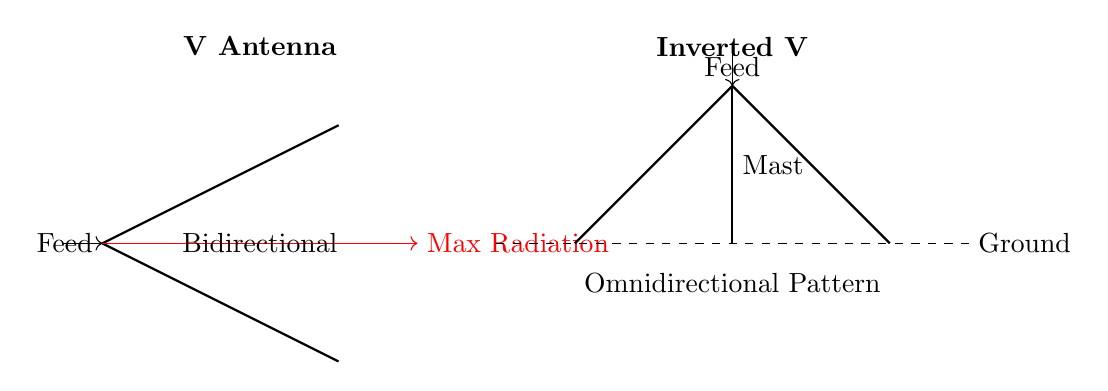
\begin{tikzpicture}
    % V Antenna
    \begin{scope}[shift={(0,0)}]
        \node [font=\bfseries] at (2, 2.5) {V Antenna};
        \draw [thick] (0,0) -- (3, 1.5);
        \draw [thick] (0,0) -- (3, -1.5);
        \draw [->] (-0.5, 0) -- (0,0) node[left] {Feed};
        \draw [red, ->] (0,0) -- (4,0) node[right] {Max Radiation};
        \node at (2, 0) {Bidirectional};
    \end{scope}

    % Inverted V
    \begin{scope}[shift={(6,0)}]
        \node [font=\bfseries] at (2, 2.5) {Inverted V};
        \draw [thick] (2, 2) -- (0, 0);
        \draw [thick] (2, 2) -- (4, 0);
        \draw [thick] (2, 2) -- (2, 0) node[midway, right] {Mast}; % Support
        \draw [->] (2, 2.5) -- (2, 2) node[above] {Feed};
        \draw [dashed] (-1,0) -- (5,0) node[right] {Ground};
        \node at (2, -0.5) {Omnidirectional Pattern};
    \end{scope}
\end{tikzpicture}
\end{answerdiagram}

\begin{tabulary}{\linewidth}{|L|L|L|}
\hline
\textbf{Feature} & \textbf{V Antenna} & \textbf{Inverted V Antenna} \\ \hline
\keyword{Geometry} & Horizontal V shape parallel to ground & Vertical upside-down V shape \\ \hline
\keyword{Radiation} & Bidirectional along the bisector axis & Nearly Omnidirectional (horizontally) \\ \hline
\keyword{Construction} & Needs multiple supports & Needs only one central support (Mast) \\ \hline
\keyword{Impedance} & High (~600 $\Omega$) & Low (~50 $\Omega$) - easier match \\ \hline
\keyword{Use} & Point-to-point HF communication & Amateur radio (Ham), Limited space \\ \hline
\end{tabulary}
\end{solutionbox}

\begin{mnemonicbox}
\mnemonic{"VIVA: V Is Vertical Arrangement, Inverted V Aims downward"}
\end{mnemonicbox}


\questionmarks{4(a)}{3}{Define: (1) Reflection, (2) Refraction and (3) Diffraction}

\begin{solutionbox}
\begin{tabulary}{\linewidth}{|L|L|}
\hline
\textbf{Phenomenon} & \textbf{Definition} \\ \hline
\keyword{Reflection} & Bouncing back of waves when they strike the boundary between two media (e.g., ground, ionosphere). \\ \hline
\keyword{Refraction} & Bending of waves when they pass from one medium to another with different density/velocity. \\ \hline
\keyword{Diffraction} & Bending of waves around obstacles or spreading through openings. Allows reception behind mountains. \\ \hline
\end{tabulary}
\end{solutionbox}

\begin{mnemonicbox}
\mnemonic{"RRD: Rebounding, Redirecting, Detour"}
\end{mnemonicbox}

\questionmarks{4(b)}{4}{List HAM radio application for communication}

\begin{solutionbox}
\begin{tabulary}{\linewidth}{|L|L|}
\hline
\textbf{Application} & \textbf{Description} \\ \hline
\keyword{Emergency Comm.} & Providing vital links during disasters when cell/landlines fail. \\ \hline
\keyword{DXing} & Long-distance international communication for hobby/sport. \\ \hline
\keyword{Satellite Comm.} & Using amateur satellites (OSCAR) for relay. \\ \hline
\keyword{Digital Modes} & Text/data via radio (FT8, PSK31, RTTY). \\ \hline
\keyword{Morse Code} & Traditional CW communication (efficient for weak signals). \\ \hline
\keyword{Education} & Learning electronics and radio physics. \\ \hline
\end{tabulary}
\end{solutionbox}

\begin{mnemonicbox}
\mnemonic{"EDSDMVP: Emergency DX Satellite Digital Morse Voice Public-service"}
\end{mnemonicbox}

\questionmarks{4(c)}{7}{Explain ionosphere's layers and sky wave propagation}

\begin{solutionbox}
\textbf{Sky Wave Propagation}: Using the ionosphere (ionized upper atmosphere) to reflect signals back to Earth for long-distance (Beyond Line of Sight) communication.

\begin{answerdiagram}{Ionospheric Layers}
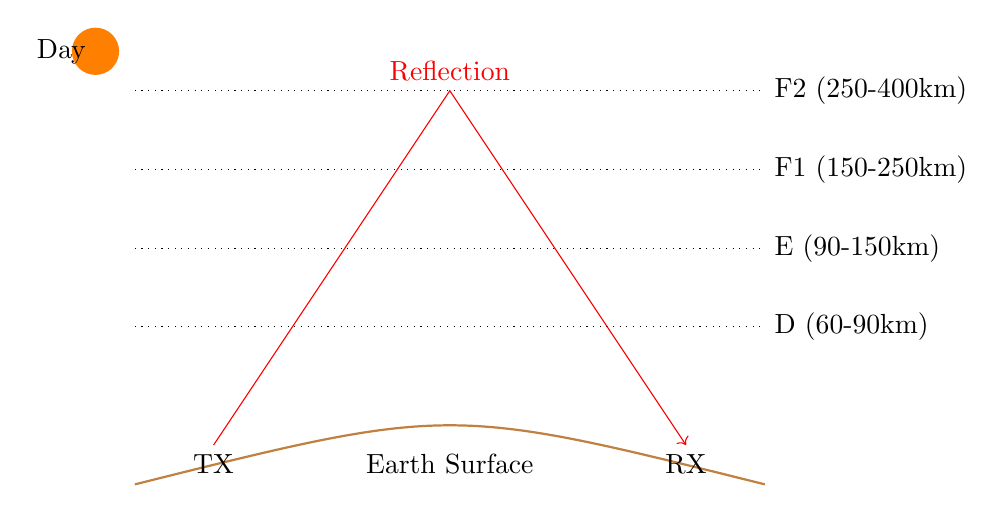
\begin{tikzpicture}
    % Earth
    \draw [thick, brown] (-4, -1) .. controls (0, 0) .. (4, -1);
    \node [below] at (0, -0.5) {Earth Surface};
    
    % Layers
    \draw [dotted] (-4, 1) -- (4, 1) node[right] {D (60-90km)};
    \draw [dotted] (-4, 2) -- (4, 2) node[right] {E (90-150km)};
    \draw [dotted] (-4, 3) -- (4, 3) node[right] {F1 (150-250km)};
    \draw [dotted] (-4, 4) -- (4, 4) node[right] {F2 (250-400km)};
    
    % Sun
    \fill [orange] (-4.5, 4.5) circle (0.3);
    \node [left] at (-4.5, 4.5) {Day};
    
    % Rays
    \draw [red, ->] (-3, -0.5) -- (0, 4) -- (3, -0.5);
    \node [red, above] at (0, 4) {Reflection};
    \node [below] at (-3, -0.5) {TX};
    \node [below] at (3, -0.5) {RX};
\end{tikzpicture}
\end{answerdiagram}

\begin{itemize}
    \item \textbf{D Layer}: Exists only during day. Absorbs MF/HF signals.
    \item \textbf{E Layer}: Reflects some HF waves. Sporadic-E allows VHF DX.
    \item \textbf{F1 Layer}: Lower part of F-region during day.
    \item \textbf{F2 Layer}: Most important for long-distance HF. Exists day and night (though height varies). Reflects highest frequencies.
    \item \textbf{Mechanism}: UV radiation from sun ionizes atoms. Radio waves enter, bend due to refraction, and return to Earth (Total Internal Reflection).
\end{itemize}
\end{solutionbox}

\begin{mnemonicbox}
\mnemonic{"DEFV: D-absorbs, E-reflects, F-provides Very-long-distance"}
\end{mnemonicbox}

\orquestionmarks{4(a)}{3}{Define: (1) MUF, (2) LUF and (3) Skip distance}

\begin{solutionbox}
\begin{tabulary}{\linewidth}{|L|L|}
\hline
\textbf{Term} & \textbf{Definition} \\ \hline
\keyword{MUF} & \textbf{Maximum Usable Frequency}: The highest f that returns to Earth for a given path. $f_{MUF} = f_c \sec\theta$. \\ \hline
\keyword{LUF} & \textbf{Lowest Usable Frequency}: The lowest f where signal > noise. Below LUF, absorption is too high. \\ \hline
\keyword{Skip Distance} & Min distance from TX where sky wave returns. Within this zone, no signal is received (Skip Zone). \\ \hline
\end{tabulary}
\end{solutionbox}

\begin{mnemonicbox}
\mnemonic{"MLS: Maximum-highest, Lowest-minimum, Skip-nearest"}
\end{mnemonicbox}

\orquestionmarks{4(b)}{4}{List HAM radio digital modes of communication}

\begin{solutionbox}
\begin{tabulary}{\linewidth}{|L|L|}
\hline
\textbf{Mode} & \textbf{Characteristics} \\ \hline
\keyword{FT8} & Weak signal mode, 15-second intervals, automated. Very popular for DX. \\ \hline
\keyword{PSK31} & Phase Shift Keying. Narrow bandwidth (31 Hz). Chat-like typing. \\ \hline
\keyword{RTTY} & Radioteletype. Robust, old-school digital text. \\ \hline
\keyword{SSTV} & Slow Scan TV. Transmitting static images via audio tones. \\ \hline
\keyword{Packet} & Data sent in packets (AX.25). Used for APRS. \\ \hline
\keyword{JT65} & Deep space/weak signal mode (precursor to FT8). \\ \hline
\end{tabulary}
\end{solutionbox}

\begin{mnemonicbox}
\mnemonic{"FIRST PAD: FT8 Is RTTY SSTV Then Packet APRS Digital-voice"}
\end{mnemonicbox}

\orquestionmarks{4(c)}{7}{Explain space wave propagation}

\begin{solutionbox}
\textbf{Space Wave (Tropospheric)}: Direct Line-of-Sight transmission for VHF, UHF, Microwave (> 30 MHz).

\begin{answerdiagram}{Space Wave Propagation}
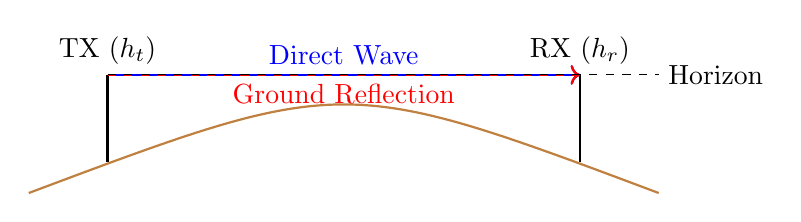
\begin{tikzpicture}
    % Earth
    \draw [thick, brown] (-4, -1) .. controls (0, 0.5) .. (4, -1);
    
    % Towers
    \draw [thick] (-3, -0.6) -- (-3, 0.5) node[above] {TX ($h_t$)};
    \draw [thick] (3, -0.6) -- (3, 0.5) node[above] {RX ($h_r$)};
    
    % Direct
    \draw [thick, blue, ->] (-3, 0.5) -- (3, 0.5) node[midway, above] {Direct Wave};
    
    % Reflected
    \draw [thick, red, dashed, ->] (-3, 0.5) -- (0, 0.5) -- (3, 0.5);
    \node [red, below] at (0, 0.5) {Ground Reflection};

    % Range
    \draw [dashed] (-3, 0.5) -- (4, 0.5) node[right] {Horizon};
\end{tikzpicture}
\end{answerdiagram}

\begin{itemize}
    \item \textbf{Components}:
    1. \textbf{Direct Wave}: Travels straight from TX to RX.
    2. \textbf{Ground Reflected}: Bounces off ground, arriving with phase delay.
    \item \textbf{Range}: Limited by curvature of Earth/Horizon.
    $$ d = 3.57 (\sqrt{h_t} + \sqrt{h_r}) \text{ km} $$
    \item \textbf{Tropospheric Scatter}: Forward scatter from turbulence allows communication slightly beyond horizon.
    \item \textbf{Ducting}: Temperature inversion traps waves, extending range to hundreds of km.
\end{itemize}
\end{solutionbox}

\begin{mnemonicbox}
\mnemonic{"DRIFT: Direct Reflection Inversion Forward Tropospheric"}
\end{mnemonicbox}

\questionmarks{5(a)}{3}{Define: (1) Beam area (2) Beam efficiency, and (3) Effective aperture}

\begin{solutionbox}
\begin{tabulary}{\linewidth}{|L|L|}
\hline
\textbf{Parameter} & \textbf{Definition} \\ \hline
\keyword{Beam Area} ($\Omega_A$) & Solid angle through which all power would radiate if intensity were constant (and equal to max). \\ \hline
\keyword{Beam Efficiency} ($\epsilon_M$) & Ratio of power in the main beam to the total radiated power (Main + Side lobes). \\ \hline
\keyword{Effective Aperture} ($A_e$) & Virtual area that captures energy from incident wave. $A_e = \frac{\lambda^2}{4\pi} G$. \\ \hline
\end{tabulary}
\end{solutionbox}

\begin{mnemonicbox}
\mnemonic{"BEA: Beam Efficiency Aperture"}
\end{mnemonicbox}

\questionmarks{5(b)}{4}{Describe need of smart antenna}

\begin{solutionbox}
\textbf{Need}: To overcome capacity limits and interference in wireless networks.

\begin{answerdiagram}{Smart Antenna Benefits}
\begin{tikzpicture}
    \node [gtu block, align=center] (center) {Smart Antenna\\Benefits};
    
    \node [gtu state, above=of center] (cap) {Capacity $\uparrow$};
    \node [gtu state, right=of center] (cov) {Coverage $\uparrow$};
    \node [gtu state, below=of center] (pwr) {Power $\downarrow$};
    \node [gtu state, left=of center] (int) {Interference $\downarrow$};
    
    \draw [gtu arrow] (center) -- (cap);
    \draw [gtu arrow] (center) -- (cov);
    \draw [gtu arrow] (center) -- (pwr);
    \draw [gtu arrow] (center) -- (int);
\end{tikzpicture}
\end{answerdiagram}

\begin{itemize}
    \item \textbf{Capacity}: SDMA (Space Division Multiple Access) allows reuse of frequencies.
    \item \textbf{Interference}: Null steering cancels out jammers/co-channel users.
    \item \textbf{Range}: High gain beams extend coverage.
    \item \textbf{Efficiency}: Transmit power is focused only where needed, saving battery.
\end{itemize}
\end{solutionbox}

\begin{mnemonicbox}
\mnemonic{"PRECISE: Power Reduction, Enhanced Coverage, Interference Suppression, Enhanced Signal"}
\end{mnemonicbox}

\questionmarks{5(c)}{7}{Draw the DTH Receiver indoor and outdoor black diagram and discuss its functions}

\begin{solutionbox}
\begin{answerdiagram}{DTH System}
\begin{tikzpicture}[node distance=1.5cm, auto]
    % Outdoor
    \node [cloud, draw, aspect=2, blue] (sat) {Satellite (Ku Band)};
    \node [draw, semicircle, rotate=90, minimum width=1cm, below=of sat] (dish) {}; 
    \node [right] at (dish) {Dish + LNB};
    \node [draw, dashed, fit=(dish), label=below:Outdoor Unit] {};

    % Indoor
    \node [gtu block, below=2cm of dish] (tuner) {Tuner};
    \node [gtu block, right=of tuner] (demod) {Demod};
    \node [gtu block, right=of demod] (dec) {Decoder};
    \node [gtu block, right=of dec] (av) {A/V Out};
    
    \node [draw, dashed, fit=(tuner) (av), label=above:Set-Top Box (Indoor)] {};

    \draw [gtu arrow, dashed] (sat) -- (dish);
    \draw [gtu arrow] (dish) -- node[left] {Coax (IF)} (tuner);
    \draw [gtu arrow] (tuner) -- (demod);
    \draw [gtu arrow] (demod) -- (dec);
    \draw [gtu arrow] (dec) -- (av);
\end{tikzpicture}
\end{answerdiagram}

\begin{itemize}
    \item \textbf{Outdoor Unit}:
    \begin{itemize}
        \item \textbf{Dish}: Parabolic reflector collects weak satellite signals (10-12 GHz).
        \item \textbf{LNB}: Downconverts high frequency to Lower IF (950-2150 MHz) for cable transmission.
    \end{itemize}
    \item \textbf{Indoor Unit (STB)}:
    \begin{itemize}
        \item \textbf{Tuner}: Selects the specific transponder frequency.
        \item \textbf{Demodulator}: Recovers digital stream (QPSK).
        \item \textbf{Decoder}: Decrypts signals (Smart Card) and decodes MPEG video.
        \item \textbf{Output}: Sends Audio/Video to TV.
    \end{itemize}
\end{itemize}
\end{solutionbox}

\begin{mnemonicbox}
\mnemonic{"COLD-TDUMS: Collection, Oscillator, Low-noise, Downconversion - Tuner Demodulator Unscrambler MPEG Smart-card"}
\end{mnemonicbox}

\orquestionmarks{5(a)}{3}{Define: (1) Antenna, (2) Folded dipole, and (3) Antenna array}

\begin{solutionbox}
\begin{tabulary}{\linewidth}{|L|L|}
\hline
\textbf{Term} & \textbf{Definition} \\ \hline
\keyword{Antenna} & A transducer that converts guided method electrical signals into free-space electromagnetic waves (and vice versa). \\ \hline
\keyword{Folded Dipole} & A dipole with an additional parallel rod connecting the two ends. Higher impedance ($300\Omega$) and wider bandwidth. \\ \hline
\keyword{Antenna Array} & A system of multiple antennas engaged to work together to achieve high directionality and gain. \\ \hline
\end{tabulary}
\end{solutionbox}

\begin{mnemonicbox}
\mnemonic{"AFA: Antenna Folded Array"}
\end{mnemonicbox}

\orquestionmarks{5(b)}{4}{Describe application of smart antenna}

\begin{solutionbox}
\begin{tabulary}{\linewidth}{|L|L|}
\hline
\textbf{Application} & \textbf{Description} \\ \hline
\keyword{Cellular (4G/5G)} & Increasing user capacity, data rates, and reducing dropped calls using Beamforming/MIMO. \\ \hline
\keyword{Wi-Fi (MIMO)} & Wi-Fi routers use multiple antennas to focus signals and improve speed through walls. \\ \hline
\keyword{Radar} & Phased arrays allow rapid scanning without moving parts (AESA radar). \\ \hline
\keyword{Satellite} & Spot beam antennas target specific geographic regions efficiently. \\ \hline
\keyword{Vehicle} & V2X communication for autonomous driving. \\ \hline
\end{tabulary}
\end{solutionbox}

\begin{mnemonicbox}
\mnemonic{"MBMRSWI: Mobile Base MIMO Radar Satellite Wi-Fi IoT"}
\end{mnemonicbox}

\orquestionmarks{5(c)}{7}{Explain Terrestrial mobile communication antennas and also discuss about base station and mobile station antennas}

\begin{solutionbox}
\textbf{Antennas in Mobile Comm}:

\begin{answerdiagram}{Mobile & Base Antennas}
\begin{tikzpicture}
    \node [gtu block] (root) {Antennas};
    
    \node [gtu block, below left=of root, xshift=-1cm] (bs) {Base Station};
    \node [gtu block, below right=of root, xshift=1cm] (ms) {Mobile Station};
    
    \node [gtu state, below=of bs] (sec) {Sectoral};
    \node [gtu state, below=of sec] (panel) {Panel};
    
    \node [gtu state, below=of ms] (pifa) {PIFA};
    \node [gtu state, below=of pifa] (whip) {Whip/Monopole};

    \draw [gtu arrow] (root) -- (bs);
    \draw [gtu arrow] (root) -- (ms);
    \draw [gtu arrow] (bs) -- (sec);
    \draw [gtu arrow] (sec) -- (panel);
    \draw [gtu arrow] (ms) -- (pifa);
    \draw [gtu arrow] (pifa) -- (whip);
\end{tikzpicture}
\end{answerdiagram}

\begin{enumerate}
    \item \textbf{Base Station Antennas (Tower)}:
    \begin{itemize}
        \item \textbf{Sector Antennas}: Vertical panels providing $120^\circ$ coverage. High gain, directional.
        \item \textbf{Omni}: Used in rural/sparse areas.
        \item \textbf{Features}: High poewr handling, weather proof, electrical tilt capability.
    \end{itemize}
    \item \textbf{Mobile Station Antennas (User)}:
    \begin{itemize}
        \item \textbf{PIFA (Planar Inverted-F)}: Used inside smartphones. Compact, low profile, multiband.
        \item \textbf{Whip/Monopole}: Used on vehicles. Omnidirectional pattern.
        \item \textbf{Requirements}: Small size, omnidirectional (to receive from any angle), low SAR.
    \end{itemize}
\end{enumerate}
\end{solutionbox}

\begin{mnemonicbox}
\mnemonic{"BEST: Base-stations Employ Sector Technology"}
\end{mnemonicbox}

\end{document}
